%%%%%%%%%%%%%%%%%%%%%%%%%%%%%%%%%%%%%%%%%%%%%%%%%%%%%%%%%%%%%%%%%%%%%%%%%%%%%%%%%%%%%%%%%%%%%%%%%%%
%%%%%%%%%%%%%%%%%%%%%%%%%%%%%%%%%%%%%%%%%%%%%%%%%%%%%%%%%%%%%%%%%%%%%%%%%%%%%%%%%%%%%%%%%%%%%%%%%%%
\section{Discusi\'on}

Como se mencion\'o en la secci\'on de hip\'otesis, este trabajo pare del supuesto en que los
sujetos con PDC presentan con mayor probabilidad estacionariedad d\'ebil en sus registros de EEG.
Esta idea fue sugerida por Cohen \cite{Cohen77}, quien a su vez se refiere a trabajos anteriores
sobre regularidad estad\'stica --estacionariedad y normalidad-- sobre registros de 
EEG \cite{McEwen75,Sugimoto78,Kawabata73}. 
Si bien en estos primeros estudios se palpa la posibilidad de que los registros de EEG fueran
ruido de alg\'un tipo, esta idea se ha probado \'erronea en estudios m\'as recientes 
\cite{Klonowski09}.

Cabe entonces mencionar una segunda justificaci\'on, un poco m\'as arbitraria y personal, sobre
las hip\'otesis de este trabajo: en el trabajo de Valeria [citar] se describen
diferencias significativas entre los registros de PSG en adultos mayores con y sin PDC,
%refiri\'endose 
hall\'andose estas diferencias respecto
al exponente de Hurst ($H_\alpha$) estimado.
La cantidad $H_\alpha$, tambi\'en referida como el ''color'' de la se\~nal,
mide la ''fractalidad''\footnote{Este concepto no se
describir\'a en este trabajo, para m\'as informaci\'on ver [trabajo de Valeria]} 
de un proceso estoc\'astico y es estimado a trav\'es del
algoritmo Detrended Fluctuation Analysis (DFA); se reporta
que el exponente $H_\alpha$ es menor para registros de PSG en adultos mayores con PSG, y que es
cercano a aqu\'el calculado para un proceso de Wiener. 
Luego entonces, cabe preguntarse sobre la naturaleza exacta de las diferencias detectadas en 
el trabajo de Valeria: ¿la se\~nal analizada es ''menos compleja'' o 
s\'olo ''tiene otro color''?
De manera concreta, en este trabajo se ha hipotetizado sobre la primera posibilidad.

En cierto modo, se ha aportado evidencias suficientes para decir que no hay cambios significativos
en la porci\'on de tiempo durante la cual el registro de PSG se comporta de manera ''simple''
--es PE. Esto puede interpretarse como que --quiz\'a-- los mecanismos afectados durante el PDC no 
provocan que la se\~nal se vuelva m\'as simple desde el punto de vista estad\'istico

Cabe un comentario sobre c\'omo la evidencia exhibe al PSG como se\~nales no-estacionarias
por una porci\'on muy prque\~na de tiempo; luego, no es adecuado analizarla con m\'etodos que
supongan estacionariedad. M\'as a\'un este comentario aplica para individuos con y sin PDC, y
se acent\'ua m\'as en individuos con problemas adicionales.

\subsubsection{La inclusi\'on de sujetos}

%Con respecto a los sujetos con problemas adicionales, cabe mencionar el caso de FGH

Durante el trabajo se menciona constantemente a tres sujetos (FGH,MGG,EMT) cuyos
registros de PSG fueron analizados
% fueron considerados
pero que no son considerados dentro de las estad\'isticas; 
como se mencion\'o anteriormente,
cada uno de ellos fue exclu\'ido del
trabajo original \cite{VazquezTagle16} 
por diversos motivos, pero dieron su consentimiento informado para la etapa
de registro de sue\~no, 
debido a lo cual se decidi\'o analizar el efecto de su inclusi\'on dentro 
de los estad\'isticas.

El caso m\'as notorio es el sujeto FGH, quien padece de par\'alisis facial,
cataratas, y problemas 
no especificados en la 
hipotiroides y la columna. Seg\'un se reporta en el trabajo original,
el sujeto no inform\'o de estos padecimientos sino hasta despu\'es del registro de PSG, por lo
que su exlusi\'on se efectu\'o a posteriori.
%Si bien la metodolog\'ia presentada aqu\'i no tiene como objetivo el diagn\'ostico
%de tal padecimiento --y bajo el etendido que hay m\'etodos menos invasivos para ello--, los
%registros confirman picos inusuales 

Dentro del marco de este trabajo, son destacableslas proporciones inusuales de \'epocas PE
en el canal F4, F7, F8, FP1, FP2, FZ, tanto en sue\~no MOR como no-MOR; es notorio no s\'olo
el 100\% de \'epocas PE en FP1, sino tambi\'en el 0\% de \'epocas PE en los otros canales. 
Si bien estas diferencias extremas llamaron la atenci\'on desde el prinicpio del estudio,
las conclusiones finales son de alguna manera consistentes con los canales que presentan 
''comportamientos inusuales'' en los registros de FGH.

\begin{figure}
\centering
%\subfloat[Comparaci\'on entre \'epocas MOR (fase R)]{
%\includegraphics[width=0.95\linewidth]
%{./material170331/Comparacion_gpos_MOR.pdf} 
%}\\
\subfloat[Compilaci\'on gr\'afica de los]{
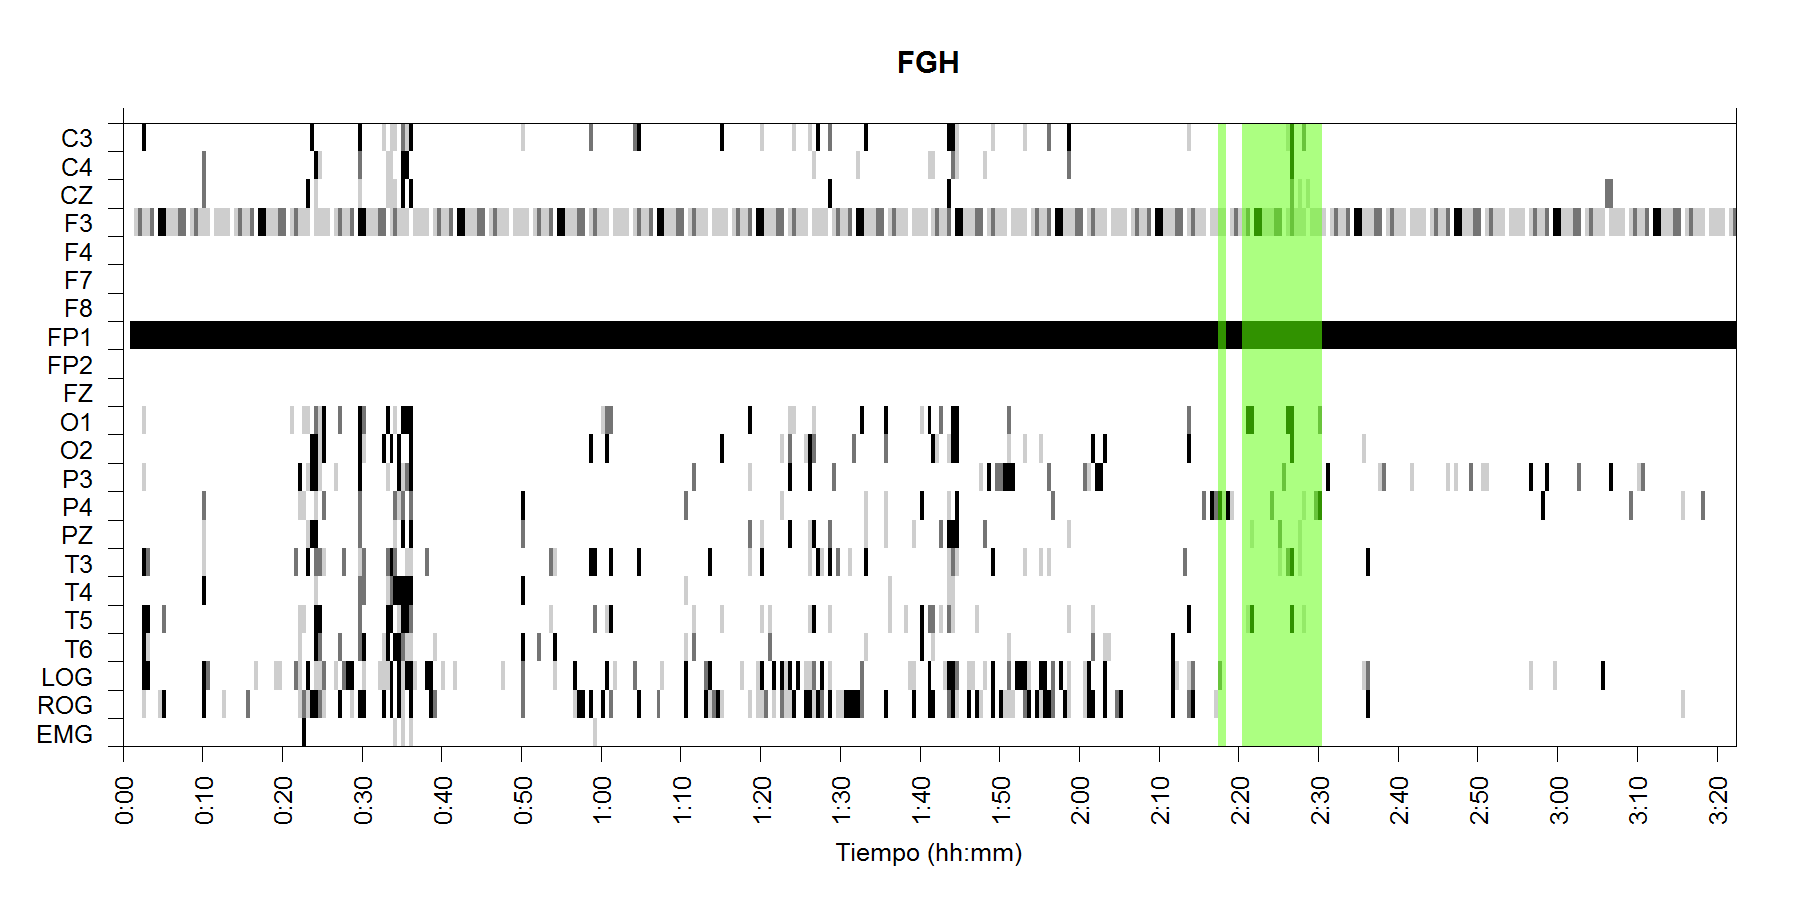
\includegraphics[width=0.95\linewidth]
{./muypreeliminar170408/FGHSUE_est.png} 
}\\
\caption{Comparaci\'on sobre las proporciones de \'epocas PE entre los grupos, para diferentes
etapas de sue\~no; se han usado los datos calculados con la segmentaci\'on de los
registros en \'epocas de 30s y 10 s replicando un detalle t\'ecnico.}
\label{FGH_especial}
\end{figure}

%\begin{comment}
%\subsubsection{Otros estimadores espectrales}
%
%Cabe mencionar que una motivaci\'on muy fuerte para utilizar el test PSR para detectar 
%estacionariedad d\'ebil, tiene su origen en el objetivo informal de
%''usar un m\'etodo previamente validado, f\'acil de
%usar e interppretar, y que se encuentre implementado en software de f\'acil acceso''.
%Este anhelo parece cumplido usando la functi\'on \texttt{stationarity} del paquete
%\texttt{fractal}, en el software estad\'istico multiplataforma, gratuito y de c\'odigo abierto 
%\texttt{R} --al menos en el \'ultimo punto.
%
%Sin embargo, dado que la prueba PSR fue mostrada por primera vez en 1969 \cite{Priestley69}, es
%intuitivo que debieran existir enfoques ''m\'as actuales''. En ese sentido
%se puede hablar, por ejemplo, de la estimaci\'on del espectro que en este trabajo se realiz\'o a
%trav\'es del estimador de doble ventana; un enfoque m\'as moderno que
%cabe destacar
%con mucho \'enfasis es
%la familia de estimadores que satisfacen una serie depropiedades descritas por Cohen 
%\cite{Cohen89} y que son referidos
%como \textbf{la clase de Cohen}.
%Esta clase puede ser interpretada como una ''suavizaci\'on'' del espectrograma, de forma similar al
%uso de la ventana espectral; su uso parece m\'as adecuado para 
%funciones 
%deterministas cuyo espectro cambia en el tiempo, y se ha generalizado su uso para procesos 
%d\'ebilmente estacionarios. 
%El autor desconoce si existe alguna generalizaci\'on
%para espectros de procesos estoc\'asticos.
%%, pero se pueden exhibir trabajos donde se usan para
%%calcular el espectro de realizaciones de procesos que presuponene como aleatorios [citar].
%M\'as a\'un, un enfoque m\'as reciente se basa en la definici\'on de estacionariedad local
%\end{comment}

%\begin{figure}
%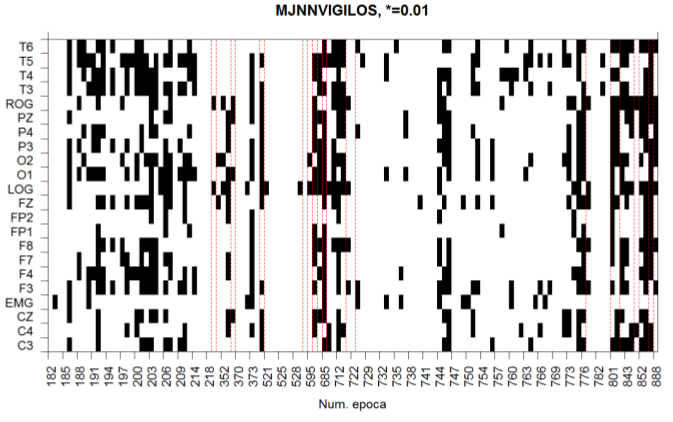
\includegraphics[width=\textwidth]{est02.png} 
%\caption{En este gráfico sólo se ilustran épocas MOR. Las líneas punteadas separan bloques continuos.
%Total de épocas: 1032 , Épocas MOR: 127}
%\label{ejemplo2}
%\end{figure}

%Para revisar si es plausible la intenci\'on de identificar las etapas de sue\~no MOR usando el
%m\'etodo gr\'afico,
%% --que eventualmente ser\'ia automatizado--
%se compar\'o la proporci\'on
%de \'epocas PE para cada sujeto dentro y fuera del sue\~no MOR usando una prueba t de Student 
%pareada --se interpreta que un sujeto cambia de ''estado'' estando o no en sue\~no MOR.
%Los p-valores se listan en la tabla \ref{apoio}
%si bien s\'olo hay diferencias significativas en LOG y ROG, estas diferencias son consistentes
%en los grupos y concuerdan con la caracterizaci\'on fisiol\'ogica del sue\~no MOR (movimientos
%ocuñares r\'apidos).


%\begin{table}
%\centering
%{\small
%\begin{tabular}{c|cccc|cccc}
%& Gpo. Normal &&&& Gpo. PDC &&&\\
%\hline
%&MOR vs NMOR&&MOR vs TOTAL&&MOR vs NMOR&&MOR vs TOTAL& \\
%\hline
%\hline
%C3&0.87&&0.87&&0.65&&0.69& \\
%C4&0.84&&0.86&&0.63&&0.68& \\
%CZ&0.96&&0.97&&0.93&&0.94& \\
%F3&0.60&&0.62&&0.52&&0.57& \\
%F4&0.62&&0.64&&0.68&&0.73& \\
%F7&0.21&&0.28&&0.40&&0.43& \\
%F8&0.35&&0.38&&0.58&&0.59& \\
%FP1&0.18&&0.20&&0.38&&0.40& \\
%FP2&0.19&&0.23&&0.42&&0.46& \\
%FZ&0.66&&0.66&&0.57&&0.61& \\
%O1&0.94&&0.94&&0.81&&0.83& \\
%O2&0.94&&0.95&&0.71&&0.75& \\
%P3&0.98&&0.98&&0.93&&0.95& \\
%P4&0.90&&0.92&&0.83&&0.85& \\
%PZ&0.88&&0.88&&0.92&&0.93& \\
%T3&0.66&&0.69&&0.77&&0.81& \\
%T4&1.00&&0.99&&0.66&&0.70& \\
%T5&0.93&&0.94&&0.76&&0.79& \\
%T6&0.94&&0.95&&0.75&&0.77& \\
%LOG&0.01&**&0.01&*&0.01&**&0.01&* \\
%ROG&0.02&* &0.03&*&0.01&*&0.02&* \\
%EMG&0.90&&0.91&&1.00&&0.98&
%\end{tabular}
%}
%\caption{Resultados de aplicar el test t de Student para muestras pareadas, a la
%proporci\'on de \'epocas PE en todos los sujetos en distintas etapas de sue\~no}
%\label{apoio}
%\end{table}

%Me siento particularmente orgulloso
%de haber dise\~nado este tipo de gr\'aficos, ya que  organizan datos que ya se ten\'ian
%y dejan la sensaci\'on de portar nueva informaci\'on.

%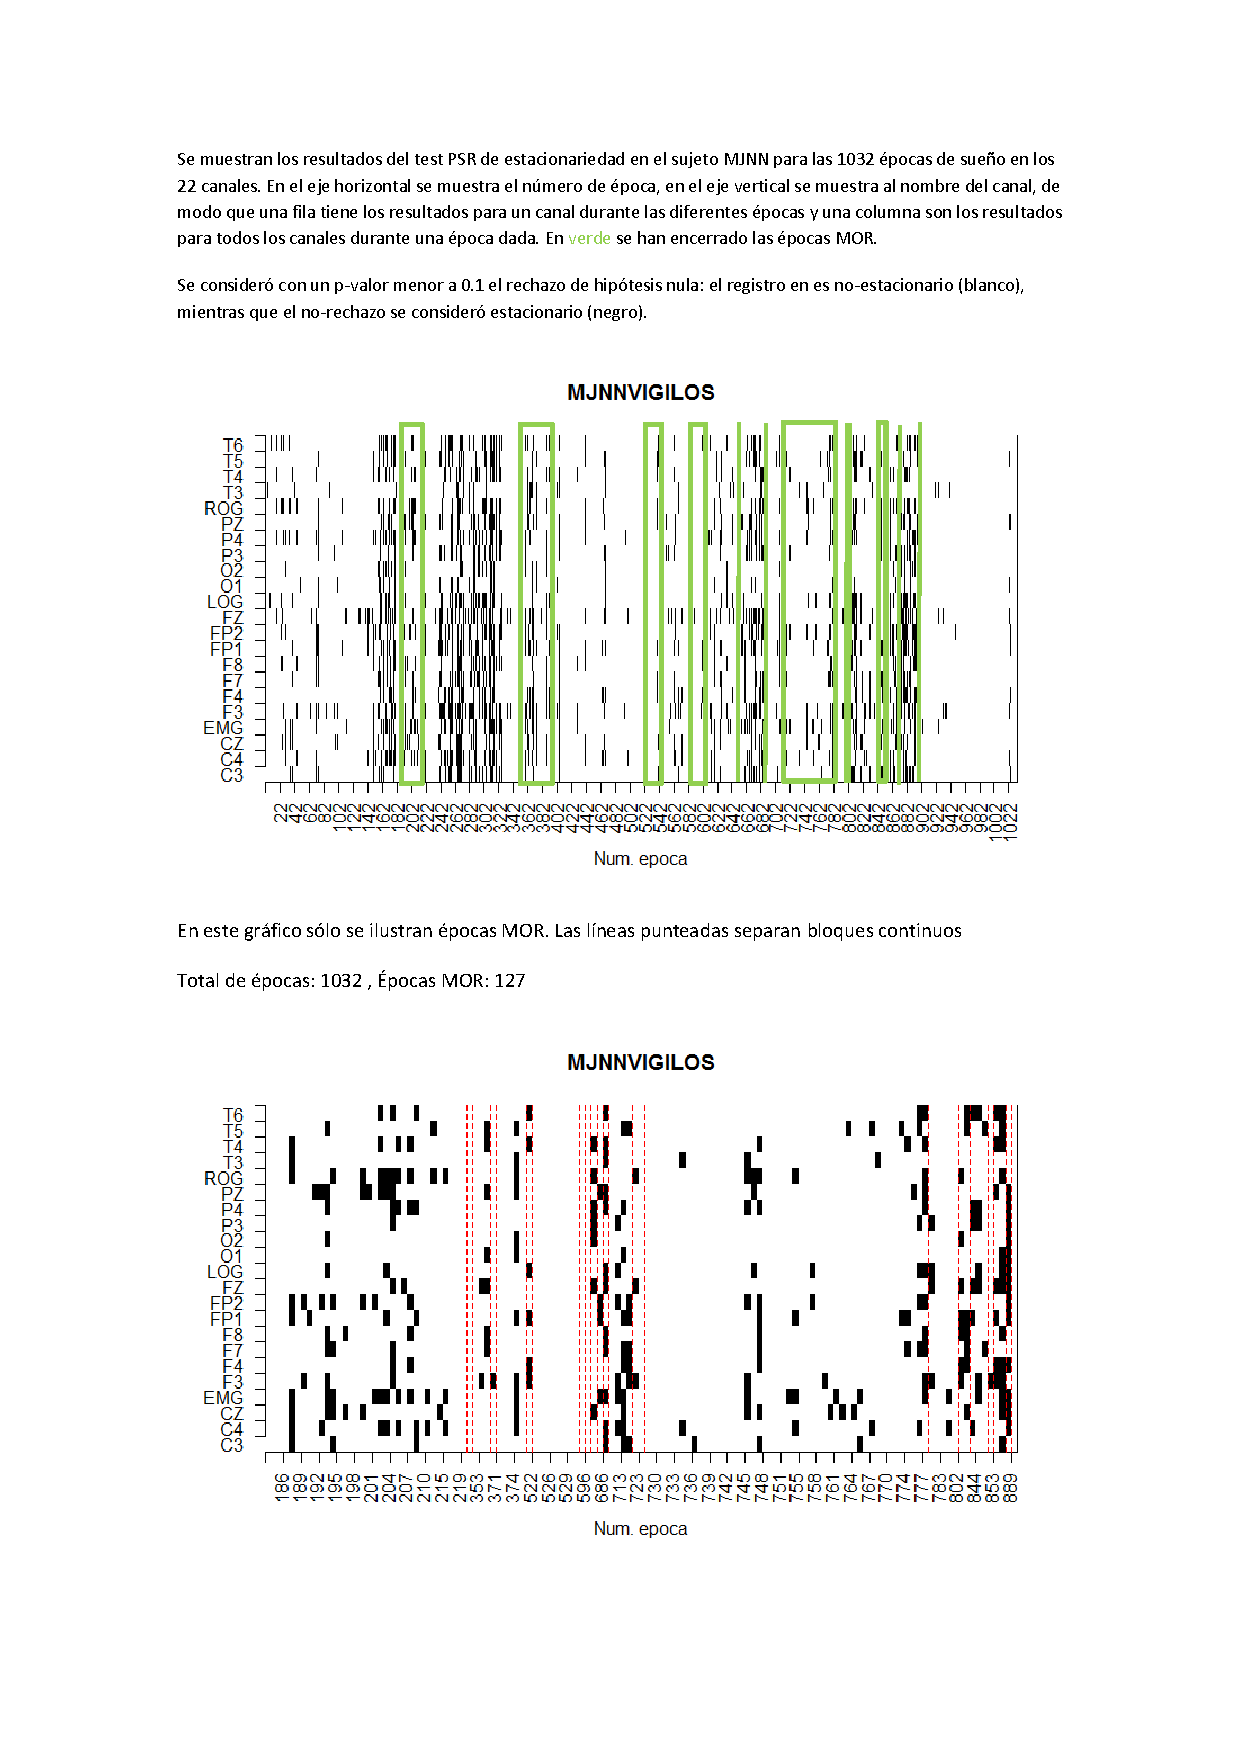
\includepdf[pages={1-},scale=.85]{reporte_de_estacionariedad_170120.pdf}
%
%\afterpage{%
%    \clearpage% Flush earlier floats (otherwise order might not be correct)
%    \thispagestyle{empty}% empty page style (?)
%    \begin{landscape}% Landscape page
%        \centering % Center table
%        \begin{figure}
%            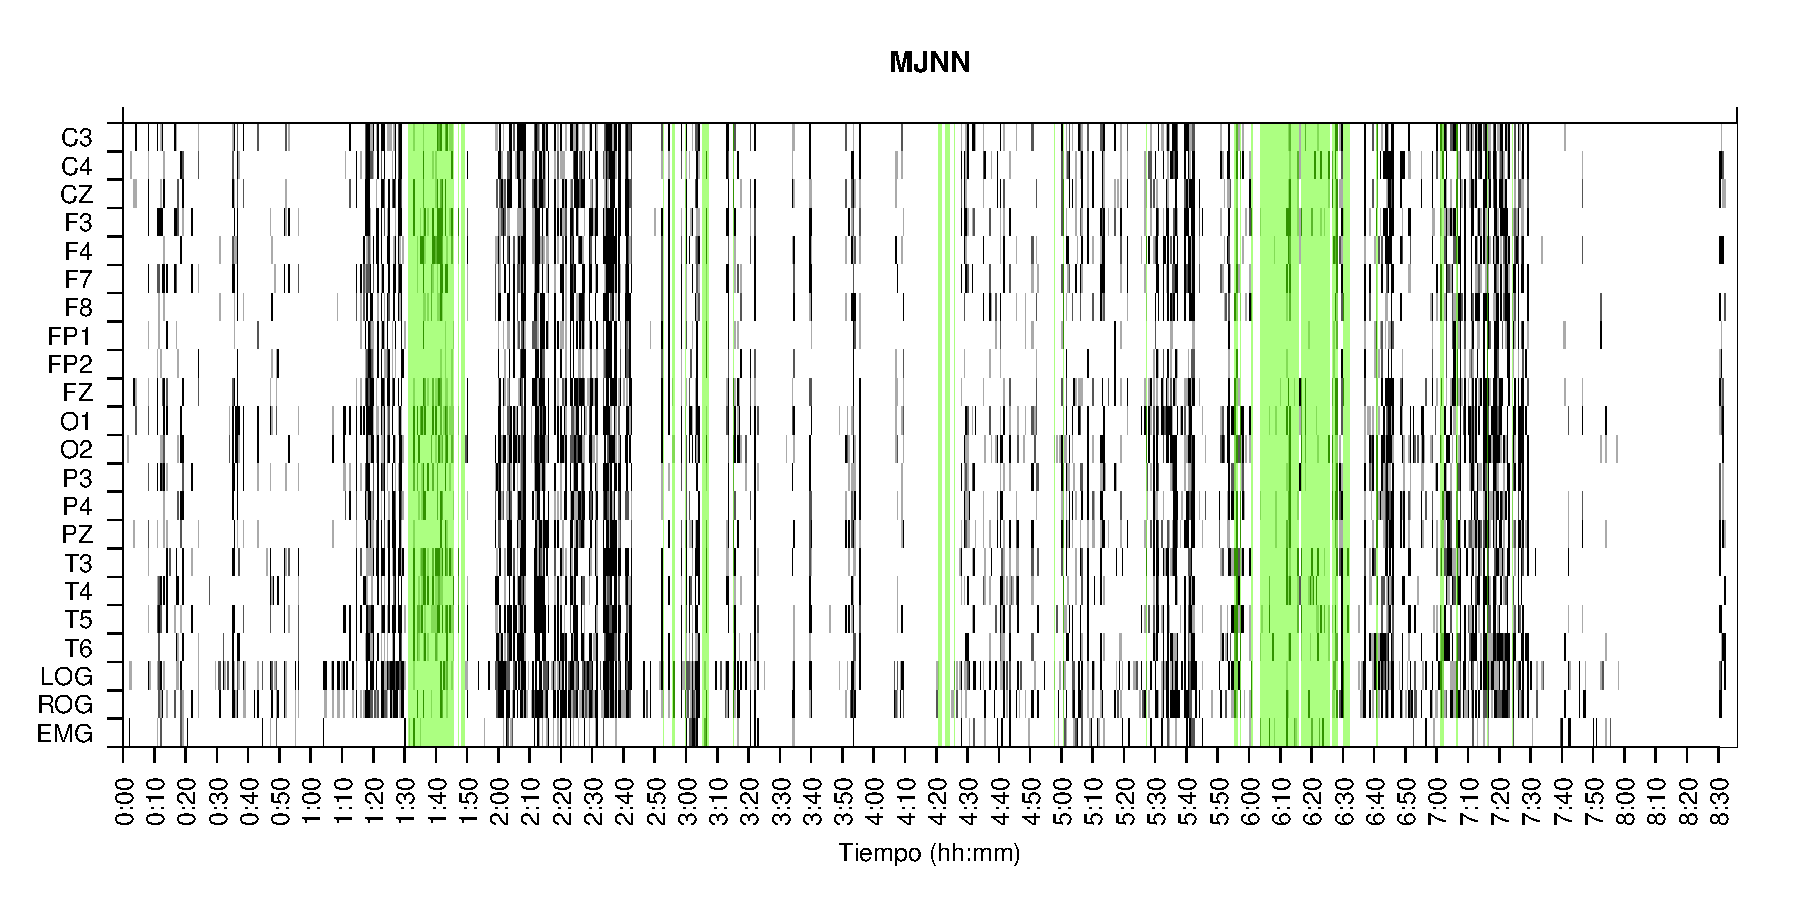
\includegraphics[width=\textwidth]{MJNNVIGILOS_127_mor127_tot1032_esttotal.pdf} 
%            \caption{Total de \'epocas: 1032, \'epocas MOR: 127}
%            %\label{ejemplo1}
%        \end{figure}
%    \end{landscape}
%    \clearpage% Flush page
%}

%%%%%%%%%%%%%%%%%%%%%%%%%%%%%%%%%%%%%%%%%%%%%%%%%%%%%%%%%%%%%%%%%%%%%%%%%%%%%%%%%%%%%%%%%%%%%%%%%%%
%%%%%%%%%%%%%%%%%%%%%%%%%%%%%%%%%%%%%%%%%%%%%%%%%%%%%%%%%%%%%%%%%%%%%%%%%%%%%%%%%%%%%%%%%%%%%%%%%%%

\subsection{Efecto del tama\~no de las \'epoca}

Debido a un problema t\'ecnico, en alg\'un momento de este trabajo se usaron los registros
de PSG segmentados en \'epocas de 10 segundos de duraci\'on.
%; aquellos sujetos cuyo PSG fue
%registrado a 200 Hz .
Al hacer los tres an\'alisis descritos anteriormente, pero con esta segmentaci\'on mixta, se 
obtuvieron resultados seg\'un los cuales no hay diferencias significativas entre los grupos
control y PDC. Estos resultados se muestran en las gr\'aficas \ref{comparacion_graf_mixto}.

\begin{figure}
\centering
\subfloat[Comparaci\'on entre \'epocas MOR (fase R)]{
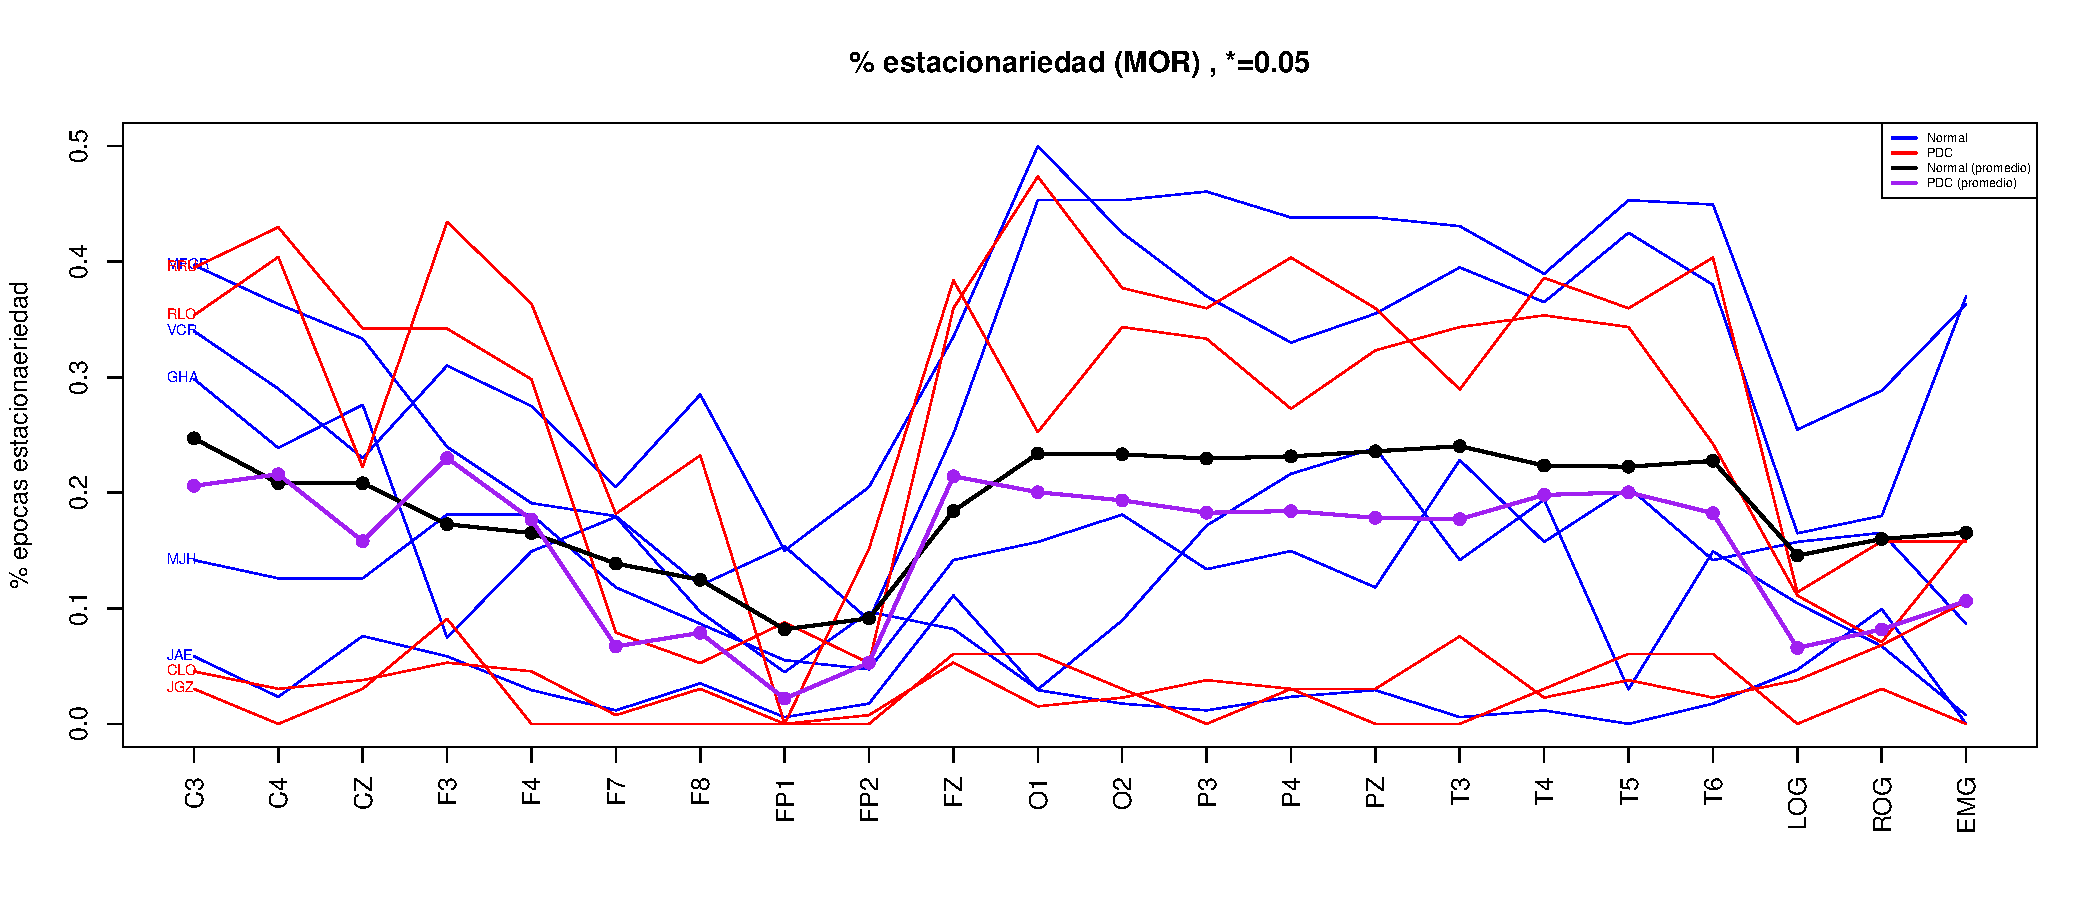
\includegraphics[width=0.95\linewidth]
{./material170331/Comparacion_gpos_MOR.pdf} 
}\\
\subfloat[Comparaci\'on entre \'epocas no-MOR (fases W y N)]{
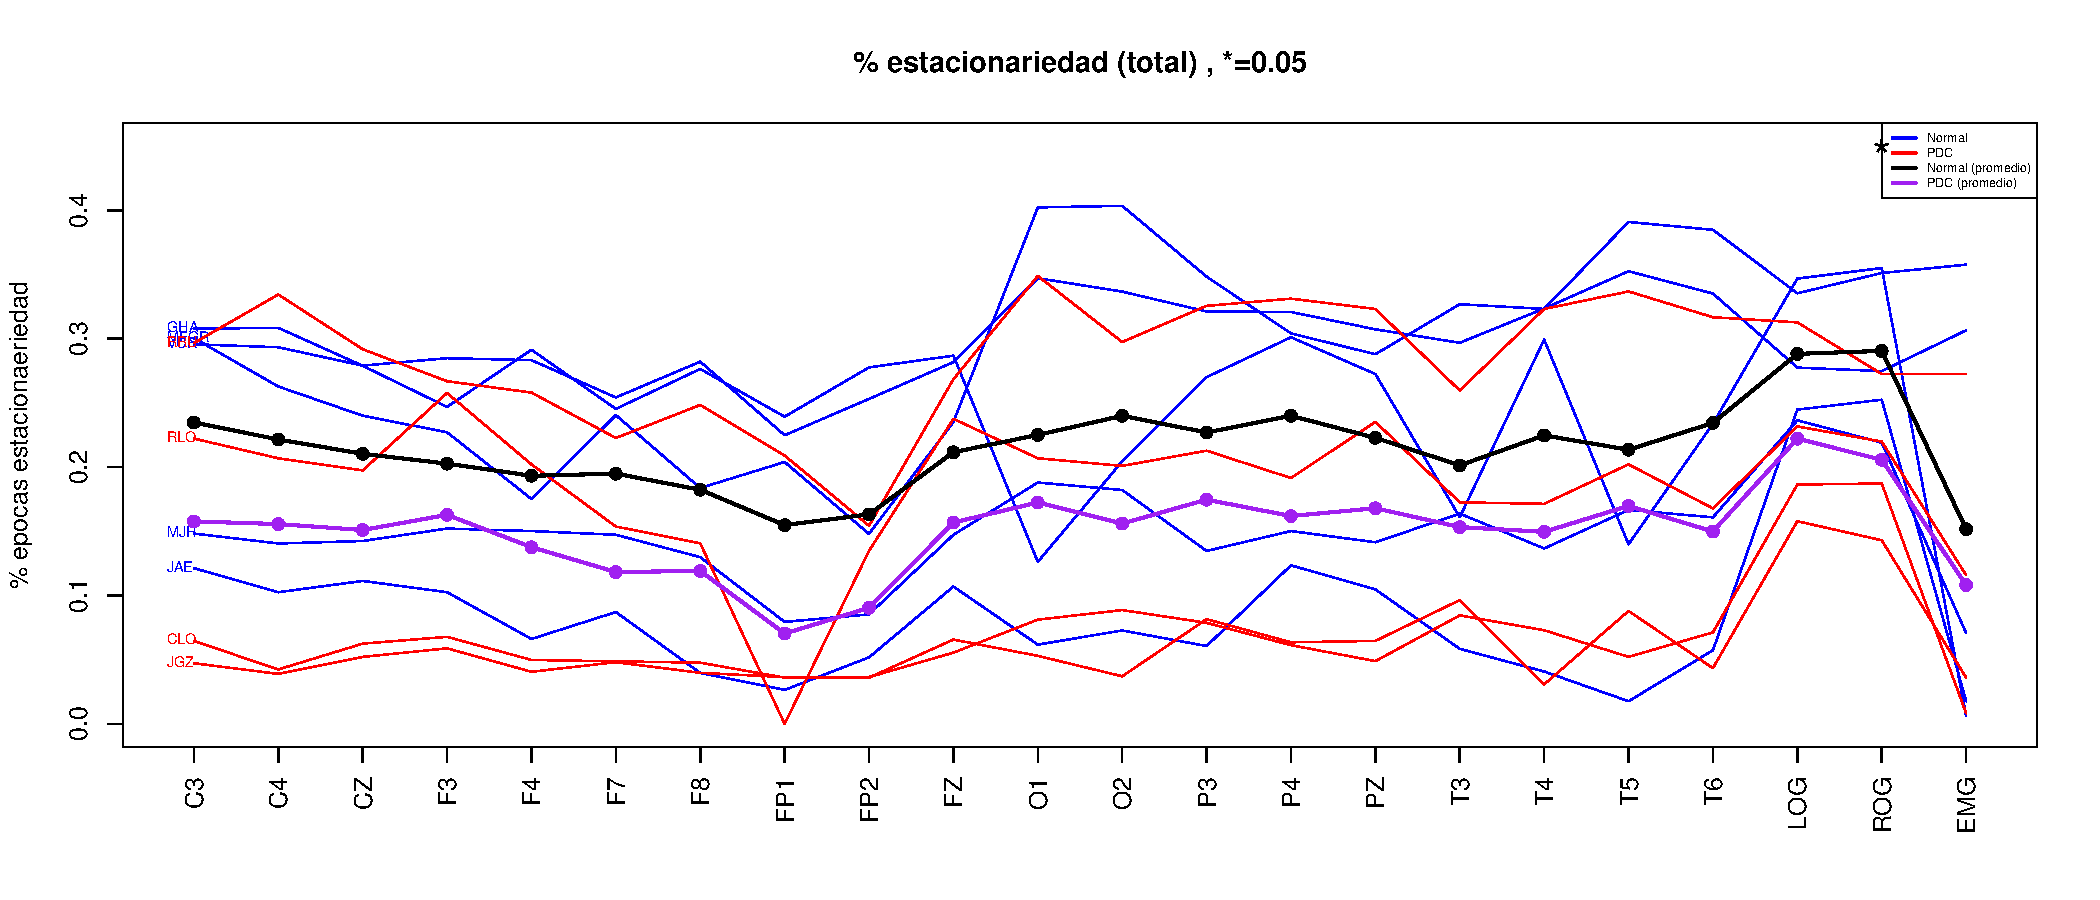
\includegraphics[width=0.95\linewidth]
{./material170331/Comparacion_gpos_NMOR.pdf} 
}\\
\caption{Comparaci\'on sobre las proporciones de \'epocas PE entre los grupos, para diferentes
etapas de sue\~no; se han usado los datos calculados con la segmentaci\'on de los
registros en \'epocas de 30s y 10 s replicando un detalle t\'ecnico.}
\label{comparacion_graf_mixto}
\end{figure}

El hecho de que los resultados encontrados sean afectados de manera contundente
por la forma en que se segmentan los
datos, merece prestar atenci\'on a la naturaleza de las diferencias encontradas y su 
posible interpretaci\'on en la fisiolog\'ia del problema.

El uso de \'epocas de 30 segundos est\'a motivado por las recomendaciones de la AAMS para 
clasificar de manera estandarizada las etapas de sue\~no --en particular el sue\~no MOR-- 
a partir de registros de PSG \cite{AASM07}. Cabe mencionar que 
en la literatura se han usado una gran variedad de
longitudes para observar el EEG, cada una de las cuales se ajusta a la naturaleza de los
fen\'omenos de inter\'es; en este trabajo se ha optado por proseguir los est\'andares en cuanto
al estudio del sue\~no, por fines de comparabilidad con trabajos afines.
%Las \'epocas de 10 segundos fueron consideradas debido a la disponibilidad de los datos.

No se discutir\'an en este trabajo motivaciones o evidencia para usar esta longitud de 
\'epoca en particular, ni para el caso contrario. Conviene, m\'as bien, presentar una posible
explicaci\'on sobre el cambio cualitativo de los datos al cambiar la longitud de las \'epocas
--entendida como un par\'ametro.
La hip\'otesis que se propone corresponde al enfoque manejado Adak \cite{Adak98}, 
quien describe una familia de procesos estacionarios ''a trozos'', que bien puede
formularse como la definici\'on \ref{a_trozos}. A grosso modo, un proceso no-estacionario
que cambia

\begin{defn}[Estacionariedad local]

\label{a_trozos}
\end{defn}

\begin{figure}
\centering
\subfloat[Usando \'epocas de 10 s]{
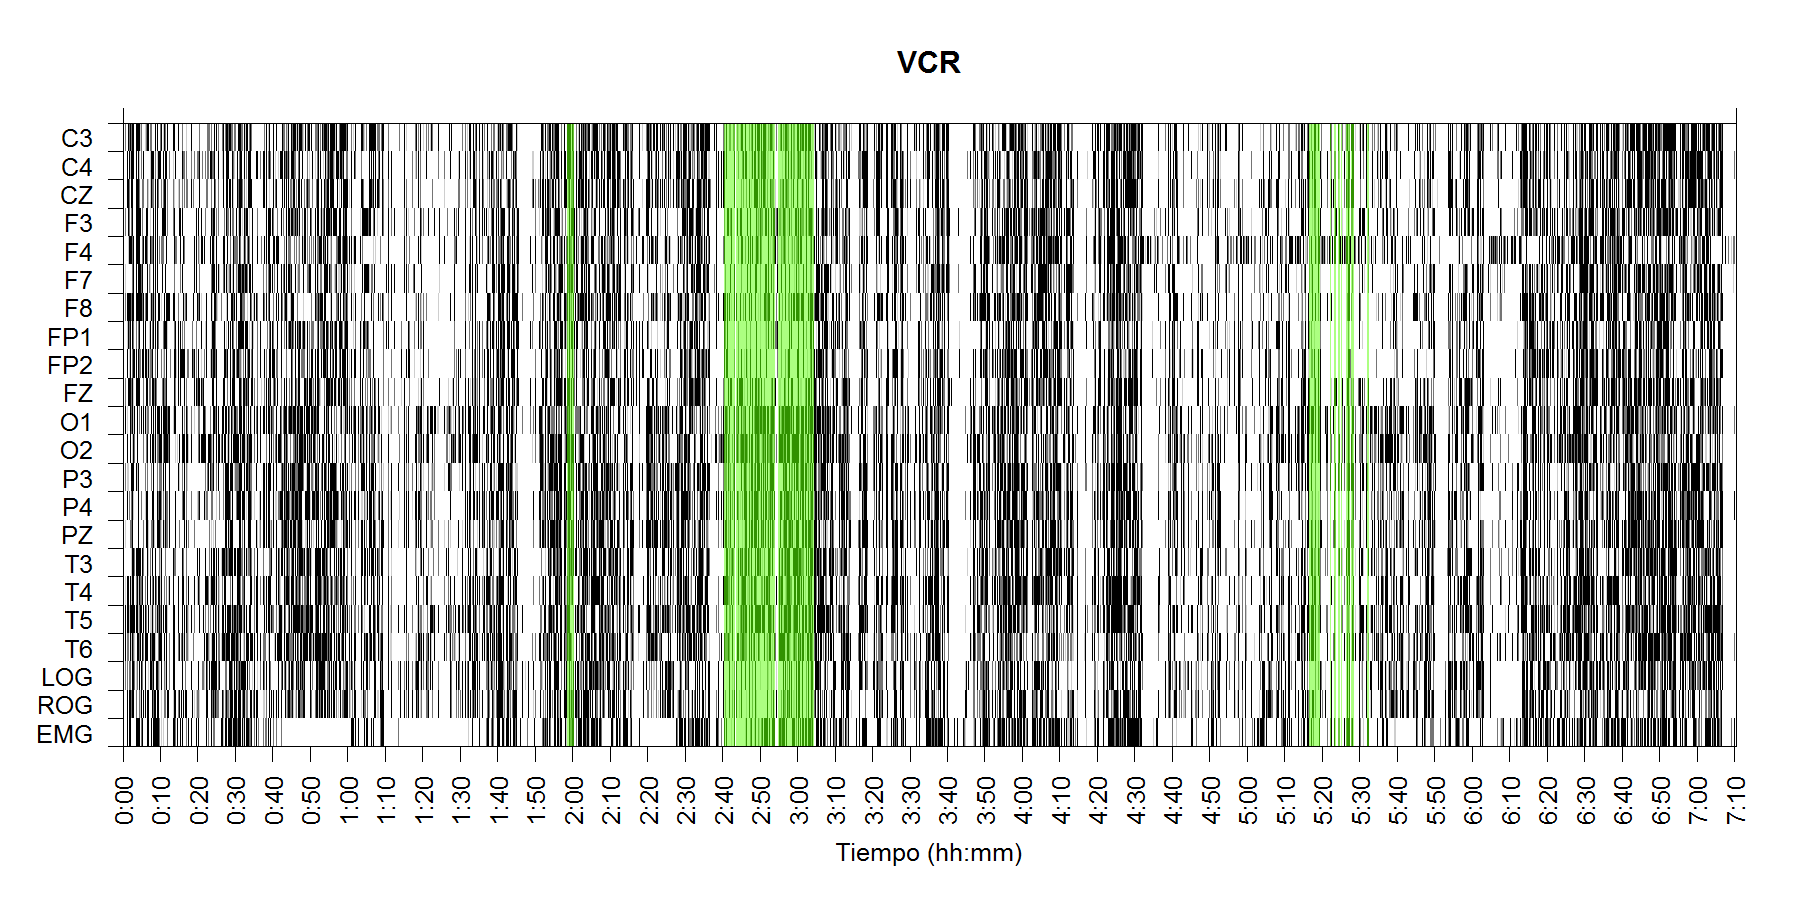
\includegraphics[width=0.95\linewidth]
{./grafiquitos170404/VCNNS1_est.png} 
}\\
\subfloat[Usando \'epocas de 30 s]{
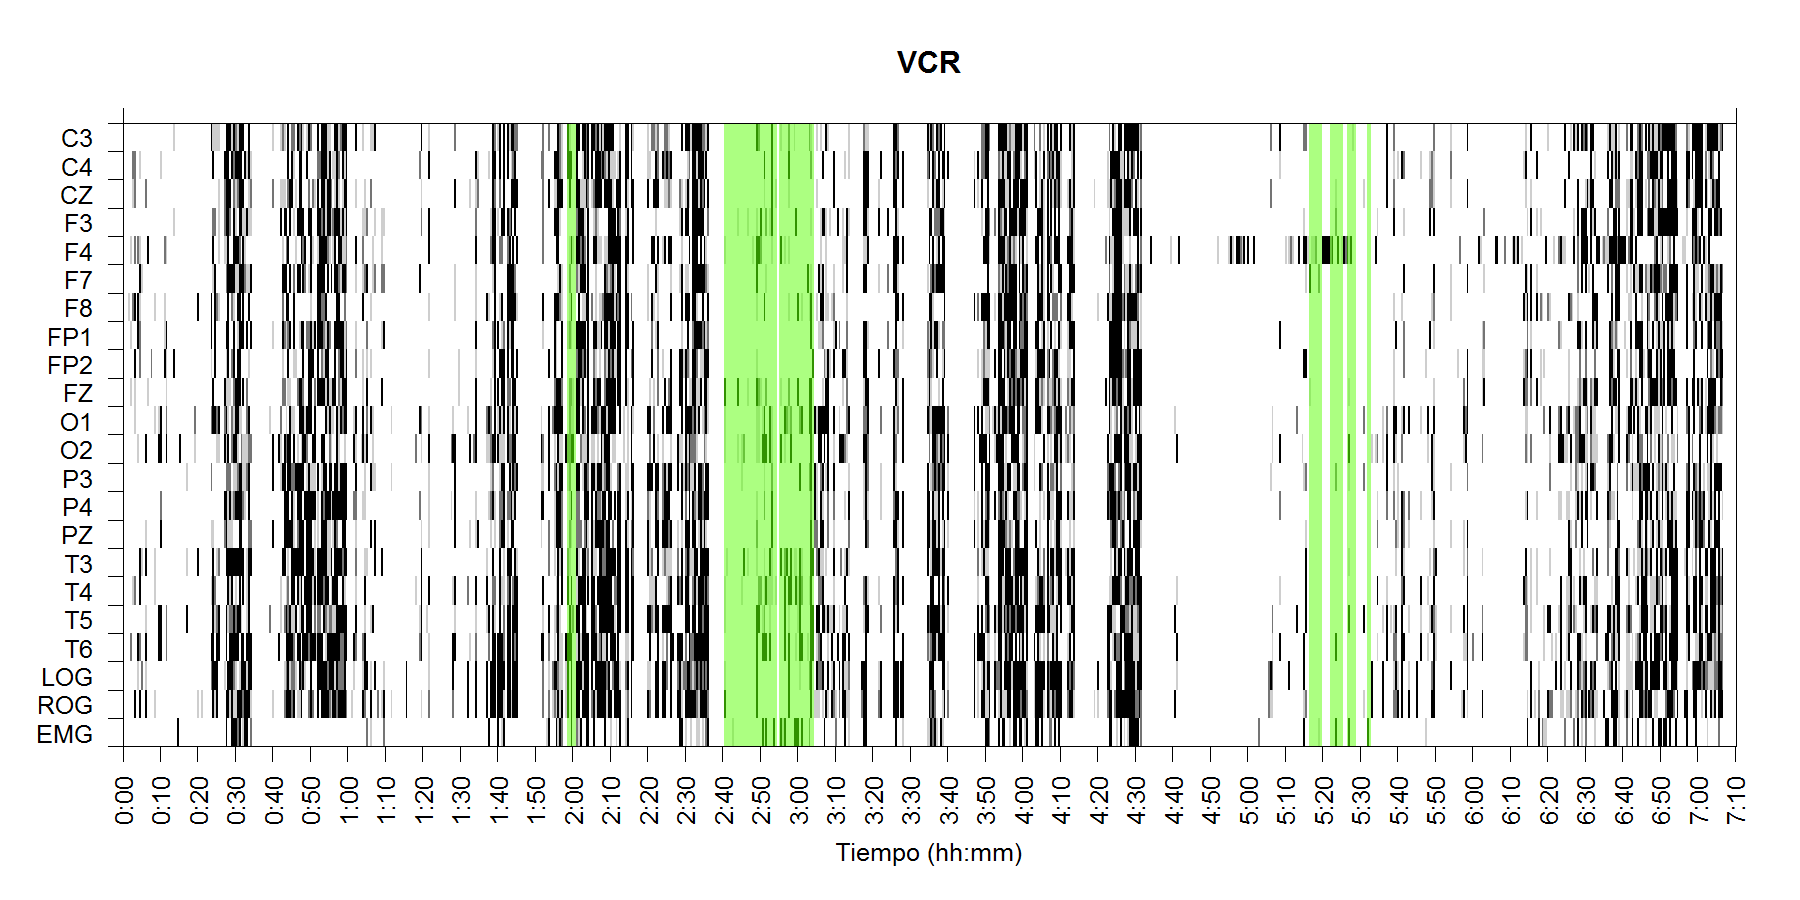
\includegraphics[width=0.95\linewidth]
{./muypreeliminar170408/VCNNS1_est.png} 
}\\
\caption{Compilaci\'on gr\'afica de las \'epocas clasificadas como PE, distribuidas en el tiempo
para cada uno de los canales. El registro corresponde al sujeto VCR dado que su registro fuera
segmentado de dos maneras difrentes, variando la duraci\'on de las \'epocas.}
\label{comp_VCR}
\end{figure}

%%%%%%%%%%%%%%%%%%%%%%%%%%%%%%%%%%%%%%%%%%%%%%%%%%%%%%%%%%%%%%%%%%%%%%%%%%%%%%%%%%%%%%%%%%%%%%%%%%%
%%%%%%%%%%%%%%%%%%%%%%%%%%%%%%%%%%%%%%%%%%%%%%%%%%%%%%%%%%%%%%%%%%%%%%%%%%%%%%%%%%%%%%%%%%%%%%%%%%%

\section{Conclusiones}

Se aportan evidencias sobre que la presencia proporcional de estacionariedad d\'ebil en registros 
de PSG para adultos mayores, segmentado en \'epocas de 30 segundos, 
presenta diferencias significativas al ser medida durante el sue\~no MOR y el resto del sue\~no
nocturno. Estas diferencia se pudieron observar, de manera grupal, 
en sujetos control para los canales 
C3, C4, F7, F8, FP1, FP2, O2, P4, LOG, ROG; en sujetos con PDC s\'olo se detectaron estas 
diferencias para los canales LOG y ROG.
%sujetos con y sin PDC diagnosticado.
%Luego entonces, esta caracter\'istica no es un indicador fiable 
Las diferencias grupales no se expresan claramente al considerar individualmente
a los sujetos excepto en los canales LOG y ROG, siendo consistente este dato con la 
caracterizaci\'on del sue\~no MOR: movimientos oculares r\'apidos y aton\'ia muscular.
Se concluye que esta caracter\'istica no es un indicador claro para ser usado
en el diagn\'ostico de PDC.

Los resultados encontrados sugieren, en cambio, que es --en principio-- posible interpretar los
cambios neurofisiol\'ogicos durante el deterioro cognitivo como un cambio en las 
en el ''mecanismo'' que genera las se\~nales del EEG, y que este cambio es detectable en el 
sue\~no nocturno mientras el sujeto transita entre las diferentes etapas del sue\~no 
(en particular, cuando transita entre el sue\~no MOR y no-MOR).
%Este cambio hipot\'etico explicar\'ia las se\~nales cualitativamente diferentes, en el sentido
%de contener una ''menor'' cantidad de cambios estructurales y eventos; la escasa presencia de 
%estas caracter\'isticas conlleva a clasificar los segmentos de registro como posiblemente
%estacionarios.
Esta interpretaci\'on propuesta es consistente con [los resultados de Valeria].

%Adicionalmente los
En otro \'ambito, los
%el hallazgos incidental de 
patrones cualitativos en el tiempo --vistos al
mostrar gr\'aficamente la distribuci\'on de \'epocas PE-- coinciden parcialmente con las \'epocas
de sue\~no MOR, clasificadas por un experto.
Adicionalmente se han encontrado diferencias significativas entre la proporci\'on de \'epocas PE,
durante sue\~no MOR y el resto del sue\~no registrado, y que son consistentes para todos los
sujetos en los canales LOG y ROG --diferencias calculadas una vez desprovista de la estructura
en el tiempo. En conjunto, se propone que la representaci\'on gr\'afica pudiera ser usado
como auxiliar en la clasificaci\'on de segmentos de registro seg\'un la etapa de sue\~no.

%%%%%%%%%%%%%%%%%%%%%%%%%%%%%%%%%%%%%%%%%%%%%%%%%%%%%%%%%%%%%%%%%%%%%%%%%%%%%%%%%%%%%%%%%%%%%%%%%%%
%%%%%%%%%%%%%%%%%%%%%%%%%%%%%%%%%%%%%%%%%%%%%%%%%%%%%%%%%%%%%%%%%%%%%%%%%%%%%%%%%%%%%%%%%%%%%%%%%%%

\section{Trabajo a futuro}

Como se ha sugerido, los patrones cualitativos hallados en la representaci\'on gr\'afica 
(''bloques de estacionariedad'') pueden tener un uso como 
caracter\'isticas auxiliares
para la detecci\'on autom\'atica de \'epocas MOR en registros de PSG.
%: el hecho que la proporci\'on
%de \'epocas PE no se vea afectada --estad\'isticamente-- por el PDC del paciente, sugiere que es
%posible obtener resultados independientes de ello. 
Para ello cabe recordar, como se mencion\'o 
en la secci\'on de discusi\'on, que en sujetos exclu\'idos de los grupos considerados, puede
que falle esta conclusi\'on: hace falta m\'as indagaci\'on al respecto. 

%Por otro lado, el uso de estimadores espectrales de ventana pueden explorarse de manera m\'as
%puntual para detectar estacionariedad sobre componentes de frecuencia espec\'ificas, de modo
%que es en principio posible separar las ondas cerebrales.

As\'i tambi\'en se mantiene a nivel de ''posiblidad'' varias de las conlcusiones mencionadas,
en cuanto a la cantidad de sujetos analizados en este trabajo es relativamente baja.
En este trabajo se han analizado tantos datos como estuvieron disponibles;
se entendie esta caracter\'istica no s\'olo como la 
capacidad real para obtener registros de PSG, sino como el conjunto de factores que conlleva
el contacto de los pacientes con las caracter\'isticas ''adecuadas'' para el estudio y su
participaci\'on voluntaria dentro del estudio bajo el marco de regulaciones \'eticas y legales 
vigentes. A esto hay que sumar el permiso para manejar estos datos en un estudio secundario,
de modo que no es realista ''exigir'' m\'as datos; a\'un as\'i, en caso de tenerlos ser\'ia
posible obtener conlcusiones estad\'isticamente m\'as generales.

%%%%%%%%%%%%%%%%%%%%%%%%%%%%%%%%%%%%%%%%%%%%%%%%%%%%%%%%%%%%%%%%%%%%%%%%%%%%%%%%%%%%%%%%%%%%%%%%%%%
%%%%%%%%%%%%%%%%%%%%%%%%%%%%%%%%%%%%%%%%%%%%%%%%%%%%%%%%%%%%%%%%%%%%%%%%%%%%%%%%%%%%%%%%%%%%%%%%%%%